\begin{figure*}[!t]
\center

\pgfplotsset{width=\textwidth,height=8cm}
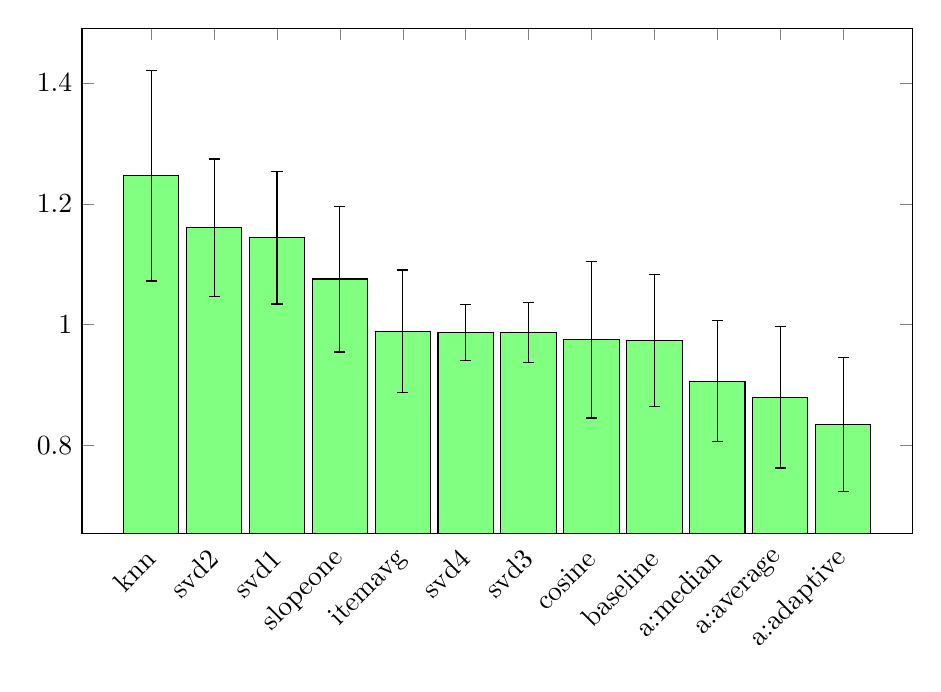
\begin{tikzpicture}

\begin{axis}[
      symbolic x coords={
        knn,svd2,svd1,slopeone,itemavg,svd4,svd3,cosine,baseline,a:median,a:average,a:adaptive},
      xtick=data,
      x tick label style={rotate=45,anchor=east,yshift=-0.5em,xshift=-0.2em},
      bar width=20pt
    ]

    \addplot [ybar,fill=green!50,error bars/.cd,y dir=both,y explicit] coordinates {
      (knn, 1.2467) +- (0,0.17435) 
      (svd2, 1.1605) +- (0,0.11385)
      (svd1, 1.1441) +- (0,0.10985)
      (slopeone, 1.0756) +- (0,0.12075)
      (itemavg, 0.9895) +- (0,0.10115)
      (svd4, 0.9873) +- (0,0.0462)
      (svd3, 0.9865) +- (0,0.04955)
      (cosine, 0.9754) +- (0,0.12975)
      (baseline, 0.9738) +- (0,0.1098)
    %};
    %\addplot [ybar,fill=blue!50] coordinates {
      (a:median, 0.9065) +- (0,0.10025)
      (a:average, 0.8801) +- (0,0.1172)
      (a:adaptive, 0.8352) +- (0,0.11125)
    };
\end{axis}

\end{tikzpicture}
\vspace{-1em}
\caption[Average RMSE Plot]{
  Average RMSE plot: This plot shows the average RMSE for each method, and each aggregation method (denoted ``a:'').
  The actual numbers are given in Table \ref{table:results:e1}.
  The error bars indicate the standard deviation of each method.
  Note the scale on the y-axis --- the errors are not as pronounced as they might seem. 
}
\label{plot:movielens}
\end{figure*}



